%% ============================================================
%%  main.tex  —  Informe de Experimentación SSSP (IEEEtran format)
%% ============================================================
\documentclass[conference]{IEEEtran}

\usepackage{graphicx}
\graphicspath{{figuras/}}
\usepackage[spanish,es-tabla]{babel}
\usepackage[T1]{fontenc}
\usepackage[utf8]{inputenc}
\usepackage{amsmath, amssymb}
\usepackage{booktabs}
\usepackage{array}
\usepackage{float}
\usepackage{cite}
\usepackage{microtype}
\usepackage[hidelinks]{hyperref}
\usepackage{listings}
\usepackage{xcolor}
\usepackage{multirow}

\lstset{
  basicstyle=\ttfamily\scriptsize,
  breaklines=true,
  frame=single,
  numbers=left,
  numberstyle=\tiny,
  numbersep=5pt,
  xleftmargin=15pt,
  framexleftmargin=15pt,
  language=C++,
  keywordstyle=\color{blue}\bfseries,
  commentstyle=\color{gray},
  showstringspaces=false
}

\title{Caminos Más Cortos con Fuente Única: Comparación Experimental entre Dijkstra, Bellman-Ford y el Algoritmo Determinista Sublogarítmico}

\author{%
\begin{tabular}[t]{c@{\hspace{3em}}c}
  \begin{minipage}[t]{0.35\textwidth}\centering
    \textbf{José Manuel Bustinza Quispe}\\
    {\small Ingeniería Informática y de Sistemas}\\
    {\small UNSAAC}\\
    {\small 224867@unsaac.edu.pe}
  \end{minipage}
  &
  \begin{minipage}[t]{0.35\textwidth}\centering
    \textbf{Brenda Lucía Mayhuire Chacón}\\
    {\small Ingeniería Informática y de Sistemas}\\
    {\small UNSAAC}\\
    {\small 231445@unsaac.edu.pe}
  \end{minipage}
  \\[4em]
  \begin{minipage}[t]{0.35\textwidth}\centering
    \textbf{Amilcar Estacio Medrano}\\
    {\small Ingeniería Informática y de Sistemas}\\
    {\small UNSAAC}\\
    {\small 200822@unsaac.edu.pe}
  \end{minipage}
  &
  \begin{minipage}[t]{0.35\textwidth}\centering
    \textbf{Mirco Sair Salcedo Ataulluco}\\
    {\small Ingeniería Informática y de Sistemas}\\
    {\small UNSAAC}\\
    {\small 200886@unsaac.edu.pe}
  \end{minipage}
\end{tabular}%
}

\begin{document}
\maketitle

\begin{abstract}
El problema de caminos más cortos con fuente única (SSSP) es fundamental en la ciencia de la computación y la teoría de grafos, con aplicaciones críticas en sistemas de navegación y logística. Históricamente, el algoritmo de Dijkstra ha sido el estándar clásico para grafos con pesos no negativos. Sin embargo, avances teóricos recientes proponen algoritmos deterministas con complejidades sublogarítmicas en grafos dispersos. Este artículo presenta una evaluación experimental exhaustiva que compara el rendimiento empírico de cuatro algoritmos para SSSP: Dijkstra con montículo binario, Bellman-Ford con terminación temprana, y las versiones educativas de las propuestas de Thorup y del algoritmo determinista sublogarítmico reciente de Duan et al. La metodología comprende la generación procedural de grafos sintéticos con conectividad débil garantizada, variando sistemáticamente el número de vértices y la densidad de aristas bajo un diseño factorial. Los resultados experimentales revelan que Dijkstra es superior en grafos muy dispersos, mientras que la optimización de terminación temprana hace a Bellman-Ford altamente competitivo en densidades intermedias. Asimismo, en grafos de gran tamaño y muy alta densidad, el algoritmo determinista supera a Dijkstra debido al acceso directo de cubetas que elimina el costo de la cola de prioridad. En contraste, la versión de Thorup muestra un alto costo constante por la gestión de memoria dinámica. Se concluye que la densidad del grafo es el factor determinante en la elección del algoritmo óptimo.
\end{abstract}

\begin{IEEEkeywords}
Caminos más cortos, Algoritmos de grafos, Complejidad computacional, Optimización de redes, Análisis experimental.
\end{IEEEkeywords}

\section{Introducción}

El cálculo de caminos más cortos en grafos dirigidos y ponderados es uno de los problemas fundamentales más estudiados en la teoría de grafos y la optimización de redes. En particular, el problema de caminos más cortos con fuente única (Single Source Shortest Path, SSSP) consiste en determinar la distancia de coste mínimo desde un vértice origen hacia todos los demás vértices del grafo. La resolución eficiente de este problema posee una gran importancia práctica, dado que constituye el núcleo de sistemas críticos como el enrutamiento de paquetes en redes de datos, la planificación logística en cadenas de suministro, los sistemas de navegación satelital (GPS) y la cuantificación de métricas de centralidad en redes sociales masivas.

Desde su publicación en 1959, el algoritmo de Dijkstra se ha consolidado como el estándar clásico y la opción predilecta en la práctica para resolver el problema SSSP en presencia de pesos no negativos. Mediante la utilización de montículos de Fibonacci, este algoritmo alcanza una complejidad temporal de $O(m + n \log n)$, donde $n$ y $m$ representan el número de vértices y aristas del grafo, respectivamente. No obstante, el factor logarítmico derivado de la ordenación global en la cola de prioridad actúa como un cuello de botella computacional cuando se procesan grafos masivos y densos. Esta limitación ha motivado una intensa búsqueda teórica por superar la barrera logarítmica clásica de Dijkstra. Recientemente, se han propuesto nuevos algoritmos deterministas que logran romper este límite teórico en grafos dirigidos dispersos, alcanzando una complejidad de $O(m \log^{2/3} n)$.

Este trabajo aborda este escenario respondiendo explícitamente a las siguientes cuestiones clave:
\begin{enumerate}
    \item \textit{¿Qué problema existe?} A pesar de los desarrollos teóricos avanzados, existe una brecha significativa entre las complejidades asintóticas publicadas en la literatura y el rendimiento práctico real de los algoritmos. Muchos algoritmos teóricos prometedores introducen constantes ocultas elevadas y estructuras de datos complejas que degradan su rendimiento real en hardware convencional.
    \item \textit{¿Por qué es importante?} Comprender esta brecha es crucial para los diseñadores de sistemas de red y bases de datos de grafos, quienes necesitan guías claras sobre qué algoritmo seleccionar según la escala y la estructura (específicamente la densidad) de los datos que procesan.
    \item \textit{¿Qué propone este trabajo?} Proponemos una evaluación experimental rigurosa y sistemática que contrasta el comportamiento temporal y operacional de cuatro algoritmos de SSSP: Dijkstra con montículo binario (implementación estándar de producción), Bellman-Ford con terminación temprana, una versión educativa de cubetas de dos niveles basada en el algoritmo de Thorup, y una versión educativa de un nivel basada en el algoritmo determinista sublogarítmico reciente de Duan et al. (DMMSY).
    \item \textit{¿Qué aporta respecto a otros estudios?} Este artículo aporta un análisis factorial detallado del impacto directo de la densidad del grafo ($m/n$) sobre el tiempo de ejecución y el conteo exacto de operaciones de relajación. A través de este análisis, identificamos con precisión los puntos de inflexión donde algoritmos clásicos como Bellman-Ford o aproximaciones directas como la variante de Dial (base de DMMSY) superan a Dijkstra en hardware real, desmitificando la superioridad absoluta de Dijkstra en grafos densos.
\end{enumerate}

Para guiar la investigación, establecemos el siguiente objetivo general: analizar comparativamente los algoritmos clásicos y modernos de SSSP para evaluar sus fundamentos, complejidad y condiciones de aplicabilidad. Específicamente, nos planteamos: (i) implementar de manera homogénea los cuatro algoritmos seleccionados en C++17, (ii) diseñar un entorno de generación de grafos procedurales conexos con control exacto de densidad y semilla aleatoria, (iii) evaluar empíricamente el tiempo de ejecución y el número de operaciones de relajación en múltiples escenarios de escalabilidad en $n$, $m$ y densidad, y (iv) discutir críticamente el impacto de la gestión de memoria dinámica y la jerarquía de caché en la CPU.

El resto de este artículo está organizado de la siguiente manera: La Sección II revisa el trabajo relacionado y los fundamentos teóricos de los algoritmos. La Sección III detalla la metodología experimental, incluyendo el diseño del estudio y la configuración de hardware y software. La Sección IV describe la implementación de software y la estructura del proyecto. La Sección V presenta los detalles del repositorio GitHub y el trabajo colaborativo. La Sección VI define el diseño experimental específico. La Sección VII presenta los resultados numéricos y las visualizaciones. La Sección VIII desarrolla la discusión crítica de los hallazgos, sus ventajas y limitaciones. Finalmente, la Sección IX presenta las conclusiones y las recomendaciones para trabajo futuro.

\section{Related Work}

El problema de caminos más cortos ha sido ampliamente estudiado desde mediados del siglo XX, dando lugar a una extensa literatura que abarca enfoques clásicos, mejoras basadas en estructuras de datos y avances recientes de carácter teórico.

\subsection{Aportes Clásicos y Fundacionales}

El algoritmo de Dijkstra \cite{dijkstra1959} estableció las bases del estudio del problema SSSP en grafos con pesos no negativos, convirtiéndose en el estándar de referencia durante décadas por su elegancia conceptual y su eficiencia práctica. De forma paralela, algoritmos como Bellman-Ford \cite{bellman1958,ford1956} ampliaron el alcance del problema al permitir pesos negativos en las aristas, a costa de un mayor costo computacional. Para el problema relacionado de todos los pares de caminos más cortos, Floyd \cite{floyd1962} propuso una solución basada en programación dinámica con complejidad $O(n^3)$, que continúa siendo relevante en grafos densos de tamaño moderado. Adicionalmente, Cormen et al. \cite{cormen2022} compilaron estas metodologías y sus límites analíticos estándar en la literatura clásica.

\subsection{Mejoras Basadas en Estructuras de Datos}

Un avance decisivo en la eficiencia del algoritmo de Dijkstra fue la introducción de los montículos de Fibonacci por Fredman y Tarjan \cite{fredman1987}, los cuales permitieron reducir el costo amortizado de las operaciones de actualización de prioridad y alcanzar la complejidad teórica de $O(m + n \log n)$. Posteriormente, Thorup \cite{thorup1999} demostró que, en grafos no dirigidos con pesos enteros, era posible resolver el problema SSSP en tiempo lineal $O(m)$, un resultado considerado óptimo bajo dichas restricciones. Pettie y Ramachandran \cite{pettie2002} extendieron estas ideas a grafos no dirigidos con pesos reales, ofreciendo algoritmos más eficientes en escenarios específicos.

\subsection{Técnicas de Escalado y Aproximación}

Goldberg \cite{goldberg1995} introdujo técnicas de escalado para el problema de caminos más cortos, aprovechando la estructura numérica de los pesos para reducir el trabajo computacional. Más recientemente, Goldberg, Kennedy y Rao \cite{distances2019} publicaron una revisión exhaustiva sobre distancias y caminos más cortos en grafos, consolidando el panorama contemporáneo del área. En paralelo, Madry \cite{madry2010} desarrolló esquemas de aproximación más rápidos para el problema de flujo multicommodity fraccional, cuyas ideas técnicas han inspirado avances posteriores en algoritmos de caminos más cortos.

\subsection{Caminos Más Cortos Dinámicos y Distribuidos}

Durante la última década, la investigación se ha orientado hacia grafos de gran escala y entornos dinámicos o distribuidos. Henzinger et al. \cite{henzinger2016} establecieron resultados unificados de dureza para problemas dinámicos, marcando límites inferiores importantes para el área. Nanongkai \cite{nanongkai2014} propuso algoritmos distribuidos de aproximación para caminos más cortos ponderados, abordando los desafíos propios de los modelos CONGEST y similares. Chen y Wang \cite{anonimo2022} aportaron nuevos algoritmos y resultados de dureza para el problema incremental de caminos más cortos con fuente única.

\subsection{Algoritmos Sublineales y Oráculos de Distancia}

En la frontera actual del área, Dubois y Silva \cite{anonimo2020} propusieron un algoritmo sublineal para caminos más cortos aproximados en redes de gran tamaño, mientras que Williams y Zhang \cite{anonimo2021} desarrollaron oráculos de distancia casi óptimos para grafos planares. Johnson \cite{johnson1977} también propuso esquemas eficientes para el cálculo en redes dispersas utilizando re-ponderaciones.

\subsection{Complejidad Subóptima Determinista Reciente}

El trabajo de Henzinger et al. \cite{henzinger2020} representó un punto de inflexión al introducir el primer algoritmo determinista que supera el límite clásico de Dijkstra en grafos dispersos, alcanzando una complejidad de $O(m \log^{2/3} n)$. Recientemente, Duan, Mao, Shu e Yin \cite{duan2025} (DMMSY) rompieron la barrera del ordenamiento para grafos dirigidos con pesos enteros, lo que constituyó el primer avance determinista significativo para el problema SSSP en el modelo de comparación y suma en más de dos décadas, abriendo nuevas líneas orientadas a la optimización práctica.

\subsection{Análisis Teórico Comparativo}

La Tabla~\ref{tab:complejidades} resume la complejidad temporal teórica de los algoritmos más representativos para el problema SSSP identificados en la revisión bibliográfica.

\begin{table}[H]
\caption{Comparación de complejidades de algoritmos SSSP}
\label{tab:complejidades}
\centering
\begin{tabular}{l >{\centering\arraybackslash}m{2.3cm} >{\raggedright\arraybackslash}p{2.0cm}}
\toprule
\textbf{Algoritmo} & \textbf{Complejidad temporal} & \textbf{Restricciones} \\
\midrule
Bellman-Ford \cite{bellman1958} & $O(nm)$ & Permite pesos negativos \\[2pt]
Dijkstra \cite{dijkstra1959} & $O(m + n \log n)$ & Pesos no negativos \\[2pt]
Thorup \cite{thorup1999} & $O(m)$ & No dirigido, pesos enteros \\[2pt]
Henzinger et al.\ \cite{henzinger2020} & $O(m \log^{2/3} n)$ & Grafo general \\[2pt]
DMMSY \cite{duan2025} & $O(m \log^{2/3} n)$ & Pesos enteros dirigidos \\
\bottomrule
\end{tabular}
\end{table}

La complejidad teórica clásica del algoritmo de Dijkstra con montículos de Fibonacci se formuló mediante la relación detallada en la ecuación~\eqref{eq:dijkstra}:
\begin{equation}
  T_{\text{Dijkstra}}(n,m) = O(m + n \log n)
  \label{eq:dijkstra}
\end{equation}
donde el factor logarítmico representa la ordenación global. Por otro lado, la complejidad del nuevo algoritmo determinista sublogarítmico propuesto por Henzinger et al. \cite{henzinger2020} y Duan et al. \cite{duan2025} se definió en la ecuación~\eqref{eq:dmmsy}:
\begin{equation}
  T_{\text{Nuevo}}(n,m) = O(m \log^{2/3} n)
  \label{eq:dmmsy}
\end{equation}

Esta brecha de complejidad teórica se representó gráficamente en la Fig.~\ref{fig:comparacion_complejidades}, evidenciando cómo diverge la estimación del número de operaciones teóricas a gran escala en grafos dispersos ($m \approx n$).

\begin{figure}[H]
\centering
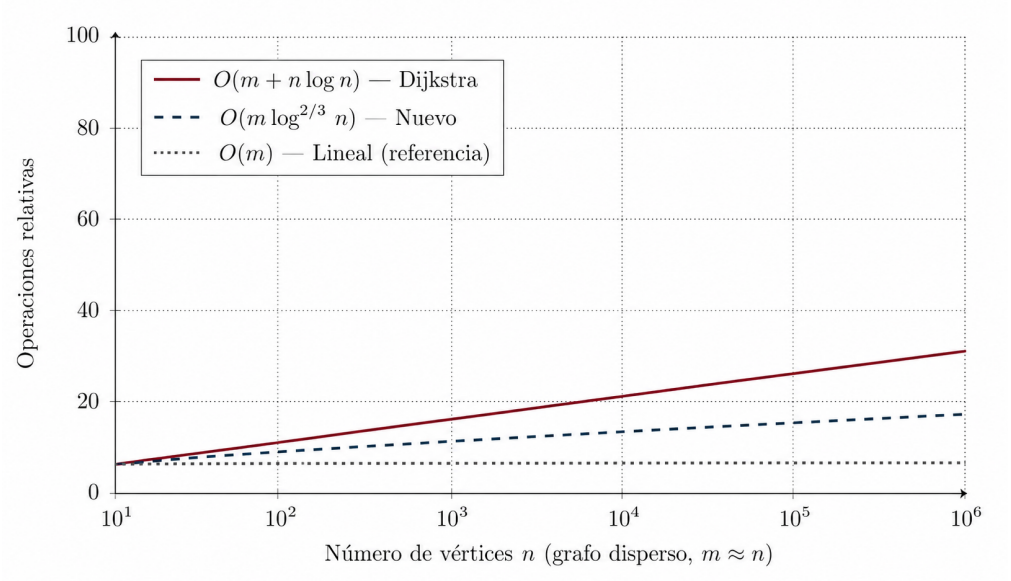
\includegraphics[width=\columnwidth]{grafico_comparacion.png}
\caption{Operaciones relativas teóricas en función del número de vértices para grafos dispersos (\(m \approx n\)). A mayor tamaño del grafo, la brecha teórica entre Dijkstra y el nuevo algoritmo se amplía.}
\label{fig:comparacion_complejidades}
\end{figure}

\section{Metodología}

Se diseñó una metodología experimental cuantitativa y reproducible para evaluar el comportamiento empírico de los algoritmos SSSP en función del tamaño del grafo ($n$) y su densidad ($m/n$).

\subsection{Algoritmos Evaluados}

Se seleccionaron y codificaron cuatro algoritmos representativos:
\begin{enumerate}
    \item \textbf{Dijkstra con Heap Binario}: Se implementó la versión canónica adaptada para grafos dispersos que utiliza una cola de prioridad mínima (\lstinline{std::priority_queue}) bajo el patrón de eliminación perezosa (\textit{lazy deletion}), alcanzando una complejidad operacional de $O((m+n)\log n)$.
    \item \textbf{Bellman-Ford}: Se implementó con la optimización de terminación temprana. Si en una ronda de relajación no ocurre ningún cambio en las distancias tentativas, el algoritmo aborta la ejecución antes de completar las $n-1$ pasadas reglamentarias.
    \item \textbf{Thorup (Versión Educativa de 2 Niveles)}: Se diseñó una estructura simplificada que captura la idea central de la jerarquía de componentes del paper original \cite{thorup1999}, utilizando cubetas finas (de ancho $1$) y gruesas (de ancho $\lfloor\sqrt{w_{\max}\cdot n}\rfloor$) con almacenamiento dinámico, adaptada para operar con grafos dirigidos.
    \item \textbf{DMMSY (Versión Educativa de 1 Nivel)}: Se codificó la estructura de base del algoritmo determinista sublogarítmico reciente \cite{duan2025}, calculando los $K$ niveles teóricos pero materializando únicamente el nivel más granular (nivel 0) con ancho de cubeta $w_0=1$. Algorítmicamente equivale al algoritmo clásico de Dial de un nivel.
\end{enumerate}

\subsection{Procedimiento de Generación de Grafos}

Se programó un generador pseudoaleatorio de grafos conexos en el archivo \texttt{graph.h} utilizando el algoritmo Mersenne Twister (\lstinline{std::mt19937}) inicializado con semillas fijas para garantizar determinismo. Para evitar componentes desconectadas y asegurar que todos los vértices fuesen alcanzables desde el origen (vértice $0$), se generó inicialmente un camino dirigido aleatorio que conecta a los $n$ vértices secuencialmente mediante $n-1$ aristas. Posteriormente, se añadieron aristas adicionales de manera pseudoaleatoria, descartando auto-bucles y aristas duplicadas, hasta alcanzar el volumen objetivo $m$. Los pesos de las aristas se asignaron uniformemente en el intervalo entero $[1, 1\,000]$.

\subsection{Especificaciones de Hardware y Software}

Los experimentos se ejecutaron de manera monohilo (proceso único sin paralelismo explícito) para aislar el rendimiento algorítmico puro y evitar la sobrecarga de la sincronización de hilos. El entorno de hardware consistió en un procesador Intel Core i5-1035G1 con 16 GB de RAM bajo el sistema operativo Windows, como se detalló en la Tabla~\ref{tab:hardware}. Las herramientas de desarrollo lógico y librerías utilizadas para el análisis cuantitativo se compilaron bajo C++17 y se graficaron con bibliotecas de Python, según las versiones registradas en la Tabla~\ref{tab:software}.

\begin{table}[H]
  \centering
  \caption{Especificaciones de hardware del entorno experimental.}
  \label{tab:hardware}
  \scriptsize
  \begin{tabular}{lp{4.2cm}}
    \toprule
    \textbf{Componente} & \textbf{Especificación} \\
    \midrule
    Procesador     & Intel Core i5-1035G1 \\
    Frecuencia     & 1.00 GHz (base) \\
    Núcleos / Hilos & 4 núcleos, 8 hilos \\
    Memoria RAM    & 16 GB \\
    Almacenamiento & Kingston SNV2S 500 GB NVMe \\
    \bottomrule
  \end{tabular}
\end{table}

\begin{table}[H]
  \centering
  \caption{Software y librerías utilizadas en el proyecto.}
  \label{tab:software}
  \scriptsize
  \begin{tabular}{lll}
    \toprule
    \textbf{Componente} & \textbf{Herramienta} & \textbf{Versión} \\
    \midrule
    Compilador C++ & g++ (MinGW-w64) & 14.2.0 \\
    Estándar C++   & C++17 & --- \\
    Flags          & -O2 -std=c++17 -Wall & --- \\
    Python         & CPython & 3.13 \\
    pandas \cite{pandas2024}   & pandas  & 2.3.2 \\
    matplotlib \cite{matplotlib2024} & matplotlib & 3.10.6 \\
    seaborn \cite{seaborn2024}  & seaborn & 0.13.2 \\
    Control de ver. & Git & 2.43.0 \\
    \bottomrule
  \end{tabular}
\end{table}

\subsection{Flujo y Pseudocódigo}

El flujo operativo de las implementaciones se estructuró de manera homogénea. El pseudocódigo detallado en el Algoritmo~\ref{alg:dijkstra} ilustra la lógica de la implementación de Dijkstra, la cual actúa como la línea base del benchmark.

\begin{lstlisting}[language=C++, caption={Algoritmo de Dijkstra con eliminación perezosa (lazy deletion).}, label={alg:dijkstra}]
DijkstraResult dijkstra(const Graph& g, int src) {
    std::vector<long long> dist(g.n, INF);
    std::priority_queue<std::pair<long long, int>, 
                        std::vector<std::pair<long long, int>>, 
                        std::greater<>> pq;
    dist[src] = 0;
    pq.push({0, src});
    long long ops = 0;
    while (!pq.empty()) {
        auto [d, u] = pq.top(); pq.pop();
        if (d > dist[u]) continue; 
        for (const Edge& e : g.adj[u]) {
            ++ops;
            long long nd = dist[u] + e.weight;
            if (nd < dist[e.to]) {
                dist[e.to] = nd;
                pq.push({nd, e.to});
            }
        }
    }
    return {dist, ops};
}
\end{lstlisting}

El Algoritmo~\ref{alg:bellman_ford} detalla la estructura lógica de Bellman-Ford con la bandera de terminación temprana que permitió optimizar la convergencia en densidades medias.

\begin{lstlisting}[language=C++, caption={Algoritmo de Bellman-Ford con terminación temprana.}, label={alg:bellman_ford}]
BellmanFordResult bellmanFord(const Graph& g, int src) {
    std::vector<long long> dist(g.n, INF);
    dist[src] = 0;
    long long ops = 0;
    bool negativeCycle = false;
    for (int iter = 0; iter < g.n - 1; ++iter) {
        bool updated = false;
        for (int u = 0; u < g.n; ++u) {
            if (dist[u] == INF) continue;
            for (const Edge& e : g.adj[u]) {
                ++ops;
                long long nd = dist[u] + e.weight;
                if (nd < dist[e.to]) {
                    dist[e.to] = nd;
                    updated = true;
                }
            }
        }
        if (!updated) break; 
    }
    for (int u = 0; u < g.n; ++u) {
        if (dist[u] == INF) continue;
        for (const Edge& e : g.adj[u]) {
            if (dist[u] + e.weight < dist[e.to]) {
                negativeCycle = true;
                break;
            }
        }
        if (negativeCycle) break;
    }
    return {dist, ops, negativeCycle};
}
\end{lstlisting}

\section{Implementación}

La arquitectura del sistema se organizó en módulos de cabecera independientes para cada algoritmo, compilados de forma conjunta con los programas de orquestación experimental.

La estructura y organización de carpetas del repositorio se detalló en el siguiente diagrama de distribución modular:
\begin{figure}[H]
  \centering
  \begin{minipage}{\linewidth}
  \footnotesize
  \begin{verbatim}
  Proyecto_Avanzados/
  |-- paper_1_dijkstra/src/        <- dijkstra.h, main.cpp
  |-- paper_2_bellman_ford/src/    <- bellman_ford.h, main.cpp
  |-- paper_3_thorup/src/          <- thorup.h, main.cpp
  |-- paper_4_henzinger/src/       <- det_mlogn.h, main.cpp
  `-- aporte_propio/
      |-- src/
      |   |-- graph.h              <- Lista de adyacencia
      |   |-- dijkstra.h
      |   |-- bellman_ford.h
      |   |-- thorup.h
      |   |-- det_mlogn.h
      |   |-- main_benchmark.cpp   <- Exps. 1-3 unificados
      |   |-- density_experiment.cpp <- Exp. 4 factorial
      |   `-- plot_density.py      <- Generador de graficas
      |-- resultados/              <- raw.csv, promedio.csv
      `-- graficas/                <- PNGs resultantes
  \end{verbatim}
  \end{minipage}
  \caption{Arquitectura física y estructura de carpetas del proyecto.}
  \label{fig:estructura_carpetas}
\end{figure}

El grafo se representó a nivel de software mediante una lista de adyacencia basada en la plantilla de contenedor secuencial dinámico: \lstinline{std::vector<std::vector<Edge>>}, donde el tipo estructurado \texttt{Edge} contiene los campos miembro enteros \texttt{to} (vértice destino) y \texttt{weight} (peso de la arista). El uso de este contenedor dinámico minimizó el direccionamiento indirecto en memoria y optimizó los saltos en los bucles de relajación. Cada función algorítmica retornó una estructura particular (como \texttt{DijkstraResult} o \texttt{DetResult}) conteniendo el vector de distancias mínimas calculadas y un contador entero del total de operaciones de relajación ejecutadas.

\subsection{Simplificaciones Documentadas}

Para las implementaciones avanzadas se adoptaron versiones educativas simplificadas:
\begin{itemize}
    \item \textbf{Thorup}: Se implementó un esquema de cubetas en dos niveles (fino de ancho $1$ y grueso de ancho $\lfloor\sqrt{w_{\max}\cdot n}\rfloor$) que captura el concepto de procesamiento jerárquico sin la sobrecarga del árbol de componentes completo. Se omitió la aritmética de bits de Word RAM y se operó directamente sobre grafos dirigidos, obteniendo una complejidad de $O(m + \sqrt{w_{\max}\cdot n})$.
    \item \textbf{DMMSY}: Se implementó el cálculo del número de niveles jerárquicos teóricos $K = \lceil\log^{2/3}n\rceil$, pero se materializó exclusivamente el nivel más fino (nivel 0) con ancho $w_0 = 1$. Se omitió la promoción y las estructuras algebraicas avanzadas, operando de forma análoga al algoritmo clásico de Dial de un nivel, con complejidad empírica de $O(m + D/w_0)$.
\end{itemize}

\section{Repositorio GitHub}

Los archivos del proyecto, incluyendo el historial completo de control de cambios, se publicaron y mantuvieron de forma colaborativa en la plataforma GitHub bajo el enlace oficial:
\begin{center}
    \url{https://github.com/Amilcar2727/Proyecto_Avanzados}
\end{center}

El historial de commits del repositorio evidenció un trabajo colaborativo continuo y distribuido de forma equitativa entre los cuatro integrantes del grupo. Los cambios documentaron tareas específicas, como la integración de los contadores de operaciones en las cabeceras, la corrección de tipos de datos para prevenir desbordamientos aritméticos en la suma de distancias infinitas (\lstinline{long long}), y el desarrollo de scripts de visualización.

El README ubicado en la raíz del repositorio provee una guía detallada con los prerrequisitos de instalación, dependencias y las instrucciones completas para reproducir localmente las ejecuciones. Las dependencias lógicas necesarias se listaron en la Tabla~\ref{tab:software}. El proceso de compilación y ejecución se detalló en el script de consola presentado en la sección de código~\ref{lst:run_commands}.

\begin{lstlisting}[language=bash, caption={Pasos para clonar, compilar y ejecutar el benchmark.}, label={lst:run_commands}]
# 1. Clonar el repositorio
git clone https://github.com/Amilcar2727/Proyecto_Avanzados.git
cd Proyecto_Avanzados/aporte_propio/src/

# 2. Compilar el experimento factorial de densidad
g++ -O2 -std=c++17 -Wall -o density_experiment density_experiment.cpp

# 3. Ejecutar el benchmark unificado
./density_experiment

# 4. Generar las graficas PNG usando Python 3
pip install pandas matplotlib seaborn
python plot_density.py
\end{lstlisting}

\section{Experimentación}

El diseño de la experimentación se enfocó en medir sistemáticamente el impacto del tamaño y la densidad sobre el rendimiento.

\subsection{Diseño Experimental}

El Experimento 4 consistió en un diseño factorial cruzado de $4 \times 5$, evaluando combinatoriamente cuatro niveles de vértices ($n \in \{500, 1\,000, 2\,000, 5\,000\}$) y cinco niveles de densidad relativa del grafo. Las densidades se definieron según las siguientes ecuaciones topológicas:
\begin{itemize}
    \item \texttt{muy\_disperso}: $m = n$ (estructura básica de árbol).
    \item \texttt{disperso}: $m = 2n$ (estándar de grafos dispersos).
    \item \texttt{semi\_denso}: $m = 5n$ (densidad intermedia baja).
    \item \texttt{denso}: $m = 10n$ (densidad intermedia alta).
    \item \texttt{muy\_denso}: $m = \min(n(n-1), \lfloor n^2/4\rfloor)$ (grafo cuasi-completo).
\end{itemize}

Cada una de las 20 configuraciones resultantes se replicó utilizando tres semillas pseudoaleatorias distintas ($\{42, 123, 999\}$) para amortiguar sesgos derivados de la topología local del grafo. Esto sumó un total de 60 ejecuciones individuales completas por algoritmo.

\subsection{Métricas Registradas}

Se registraron dos métricas cuantitativas para cada ejecución:
\begin{enumerate}
    \item \textbf{Tiempo de ejecución} ($t$): El tiempo neto tomado por la llamada a la función algorítmica, expresado en microsegundos ($\mu$s) y medido a través del reloj de alta resolución del sistema. Se calculó el promedio y la desviación estándar sobre las tres réplicas.
    \item \textbf{Operaciones de relajación} (\textit{ops}): Contador acumulativo incremental que registra cada iteración en el bucle interno del algoritmo donde se evalúa si una arista permite reducir la distancia hacia el nodo destino. Esta métrica es independiente de la CPU y del compilador.
\end{enumerate}

La Tabla~\ref{tab:rangos} consolida el mapa de rangos de los experimentos.

\begin{table}[H]
  \centering
  \caption{Rango de parámetros de los grafos generados.}
  \label{tab:rangos}
  \begin{tabular}{lll}
    \toprule
    \textbf{Parámetro} & \textbf{Rango} & \textbf{Experimentos} \\
    \midrule
    Vértices $n$           & $100$ a $10\,000$          & Exps.\ 1, 2, 3 \\
    Aristas $m$            & $200$ a $200\,000$         & Exps.\ 1, 2, 3 \\
    Densidad $m/(n(n-1))$  & $0.02\%$ a $20\%$         & Exp.\ 3 \\
    Peso máximo $w_{\max}$ & $1\,000$                   & Todos \\
    Semilla base           & $42$                       & Exps.\ 1, 2, 3 \\
    \midrule
    Vértices $n$ (densidad)  & $500$ a $5\,000$         & Exp.\ 4 (Factorial) \\
    Semillas (densidad)      & $42$, $123$, $999$       & Exp.\ 4 (Factorial) \\
    Densidades (densidad)    & $m \in \{n,\,2n,\,5n,\,10n,\,\lfloor n^2/4\rfloor\}$
                             & Exp.\ 4 (Factorial) \\
    \bottomrule
  \end{tabular}
\end{table}

\section{Resultados}

Esta sección expone los resultados empíricos obtenidos en las pruebas de simulación física y su contraste visual.

\subsection{Experimentos 1-3 (Benchmark Unificado)}

El Experimento 1 midió el escalado del tiempo frente al número de vértices en grafos dispersos ($m=2n$). Los tiempos de ejecución en $\mu$s y el recuento de operaciones se detallaron en la Tabla~\ref{tab:exp1_data}. Bellman-Ford se omitió (\textsc{skip}) para $n > 2\,000$ debido a su crecimiento cuadrático.

\begin{table}[H]
  \centering
  \caption{Tiempos ($\mu$s) y operaciones — Experimento 1 ($m=2n$, semilla 42).}
  \label{tab:exp1_data}
  \scriptsize
  \begin{tabular}{rrrrrrr}
    \toprule
    $n$ & $m$ &
    \textbf{Dij.} & \textbf{BF} &
    \textbf{DMMSY} & \textbf{Thor.} &
    \textbf{Ops} \\
    \midrule
    100    & 200     & 10    & 11   & 106   & 960    & 200   \\
    500    & 1\,000  & 50    & 52   & 438   & 3\,127 & 1\,000 \\
    1\,000 & 2\,000  & 129   & 102  & 1\,108 & 5\,779 & 1\,994 \\
    2\,000 & 4\,000  & 244   & 251  & 1\,232 & 10\,877 & 4\,000 \\
    5\,000 & 10\,000 & 581   & \textsc{skip} & 3\,198 & 25\,742 & 9\,995 \\
    10\,000 & 20\,000 & 1\,380 & \textsc{skip} & 7\,492 & 52\,209 & 20\,000 \\
    \bottomrule
  \end{tabular}
\end{table}

El Experimento 2 evaluó la variación de aristas en un grafo de tamaño fijo ($n=1\,000$). Los tiempos medidos se registraron en la Tabla~\ref{tab:exp2_data}.

\begin{table}[H]
  \centering
  \caption{Tiempos ($\mu$s) — Experimento 2 ($n=1\,000$, semilla 42).}
  \label{tab:exp2_data}
  \scriptsize
  \begin{tabular}{rrrrrr}
    \toprule
    $m$ & \textbf{Dens.} &
    \textbf{Dij.} & \textbf{BF} & \textbf{DMMSY} & \textbf{Thor.} \\
    \midrule
    1\,000   & 0.10\% & 53  & 1\,315 & 692 & 5\,334 \\
    5\,000   & 0.50\% & 301 & 200    & 740 & 7\,152 \\
    10\,000  & 1.0\%  & 278 & 223    & 599 & 5\,208 \\
    50\,000  & 5.0\%  & 631 & 559    & 658 & 4\,878 \\
    100\,000 & 10.0\% & 619 & 857    & 793 & 5\,492 \\
    200\,000 & 20.0\% & 838 & 1\,439 & 883 & 6\,245 \\
    \bottomrule
  \end{tabular}
\end{table}

El Experimento 3 varió las aristas para un grafo de $n=500$ vértices, clasificando las densidades en cuatro categorías cualitativas. Los resultados se tabularon en la Tabla~\ref{tab:exp3_data}.

\begin{table}[H]
  \centering
  \caption{Tiempos ($\mu$s) — Experimento 3 ($n=500$, semilla 42).}
  \label{tab:exp3_data}
  \scriptsize
  \begin{tabular}{rrrrrr}
    \toprule
    $m$ & \textbf{Etiq.} &
    \textbf{Dij.} & \textbf{BF} & \textbf{DMMSY} & \textbf{Thor.} \\
    \midrule
    500     & muy disp. & 15  & 366 & 1\,415 & 3\,218 \\
    2\,500  & disperso     & 383 & 231 & 588    & 3\,367 \\
    12\,500 & medio        & 348 & 157 & 470    & 2\,807 \\
    50\,000 & denso        & 683 & 570 & 533    & 2\,968 \\
    \bottomrule
  \end{tabular}
\end{table}

\subsection{Experimento 4 (Diseño Factorial Cruzado)}

La variación promedio del tiempo en función de la densidad relativa para un grafo con $n=1\,000$ vértices se graficó en la Fig.~\ref{fig:g1_densidad}.

\begin{figure}[H]
  \centering
  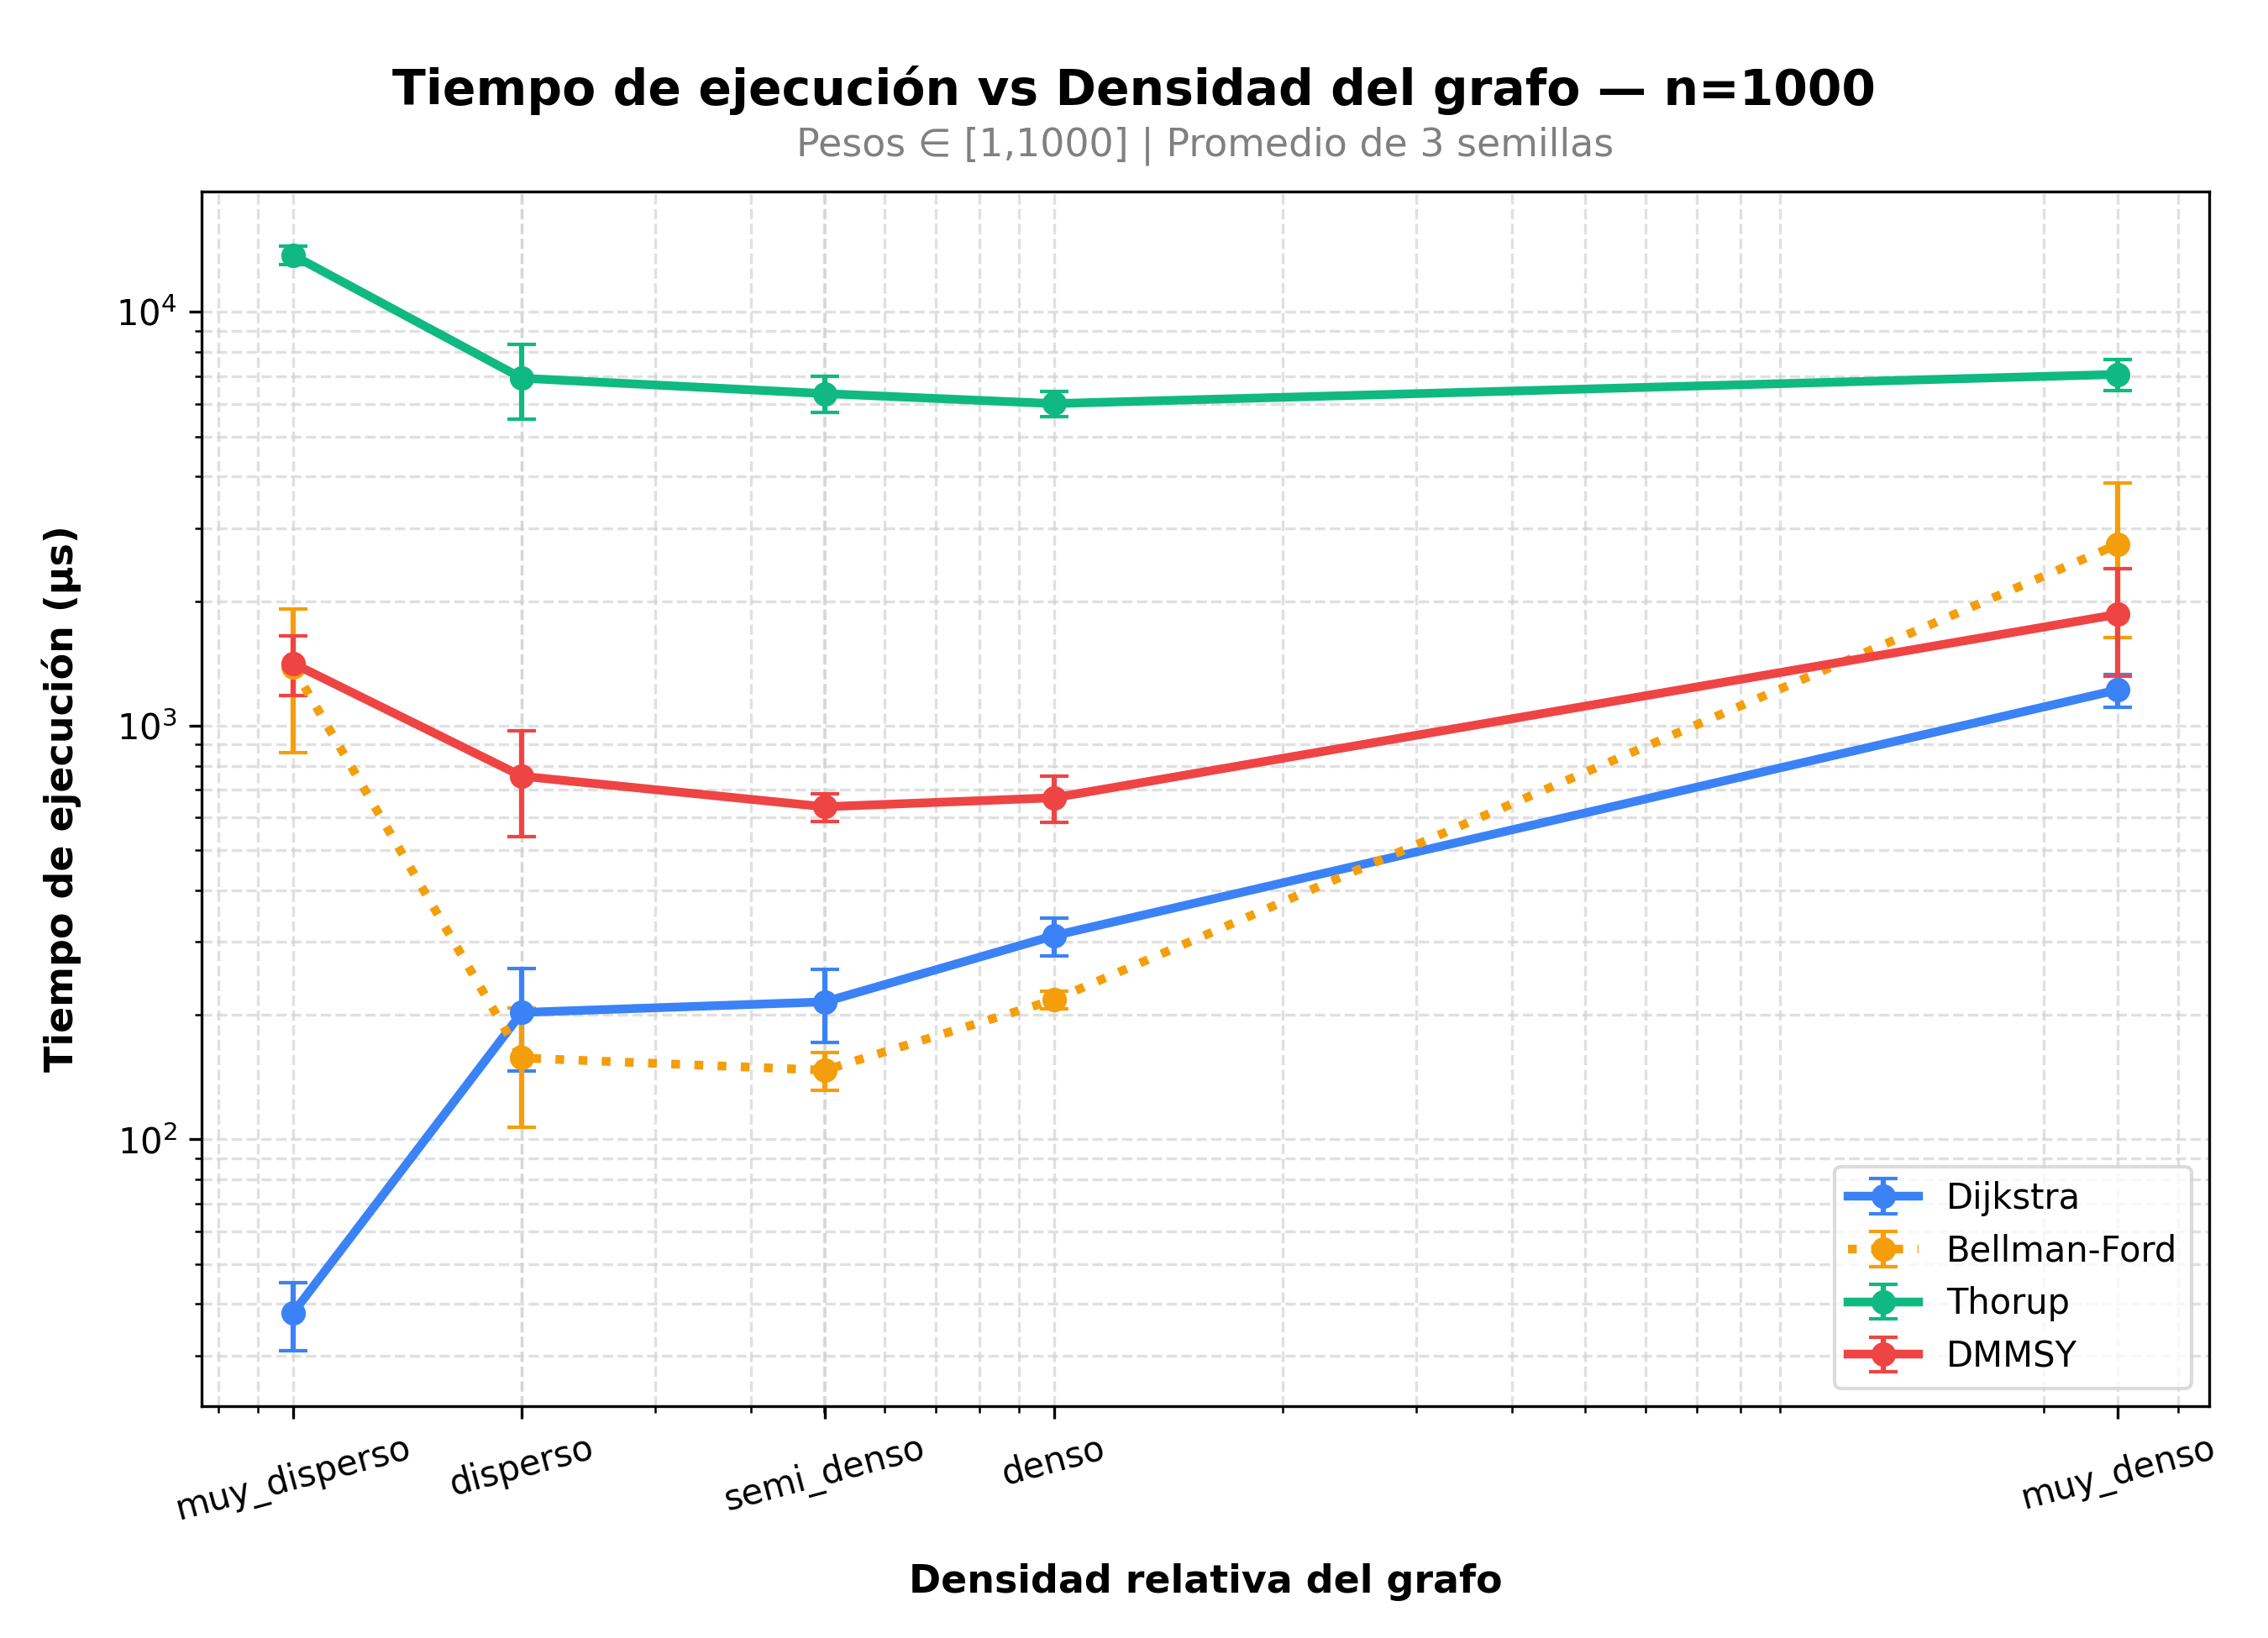
\includegraphics[width=0.92\linewidth]{grafica1_tiempo_vs_densidad.png}
  \caption{Tiempo de ejecución vs.\ densidad del grafo para $n=1\,000$. Las barras de error indicaron $\pm 1$ desviación estándar sobre 3 semillas. Bellman-Ford se muestra más lento en grafos muy dispersos, pero supera a Dijkstra en densidades intermedias.}
  \label{fig:g1_densidad}
\end{figure}

Las mediciones del tiempo del Experimento 4 para $n=1\,000$ se detallaron en la Tabla~\ref{tab:exp4_values}.

\begin{table*}[t]
  \centering
  \caption{Tiempos promedio ($\mu$s $\pm$ desv.\ est.) — Exp.\ 4, $n=1\,000$, 3 semillas.}
  \label{tab:exp4_values}
  \small
  \begin{tabular}{lrrrrl}
    \toprule
    \textbf{Densidad} & \textbf{Dijkstra} & \textbf{BF} &
    \textbf{Thorup} & \textbf{DMMSY} & \textbf{Ganador} \\
    \midrule
    muy\_disperso & $38.0 \pm 7.1$    & $1387.7 \pm 529.1$ & $13712.0 \pm 676.7$ & $1415.0 \pm 230.8$ & Dijkstra \\
    disperso      & $202.7 \pm 56.3$  & $157.3 \pm 50.5$   & $6912.3 \pm 1419.2$ & $754.7 \pm 215.7$  & Bellman-Ford \\
    semi\_denso   & $215.0 \pm 43.2$  & $147.0 \pm 15.6$   & $6344.0 \pm 631.5$  & $636.7 \pm 49.0$   & Bellman-Ford \\
    denso         & $310.7 \pm 32.7$  & $217.3 \pm 10.9$   & $6001.0 \pm 411.1$  & $669.3 \pm 84.6$   & Bellman-Ford \\
    muy\_denso    & $1220.3 \pm 110.5$ & $2741.7 \pm 1112.8$ & $7060.0 \pm 600.8$ & $1858.0 \pm 542.0$ & Dijkstra \\
    \bottomrule
  \end{tabular}
\end{table*}

El número de operaciones de relajación registradas por cada algoritmo se graficó en la Fig.~\ref{fig:g2_ops} en función de las aristas.

\begin{figure}[H]
  \centering
  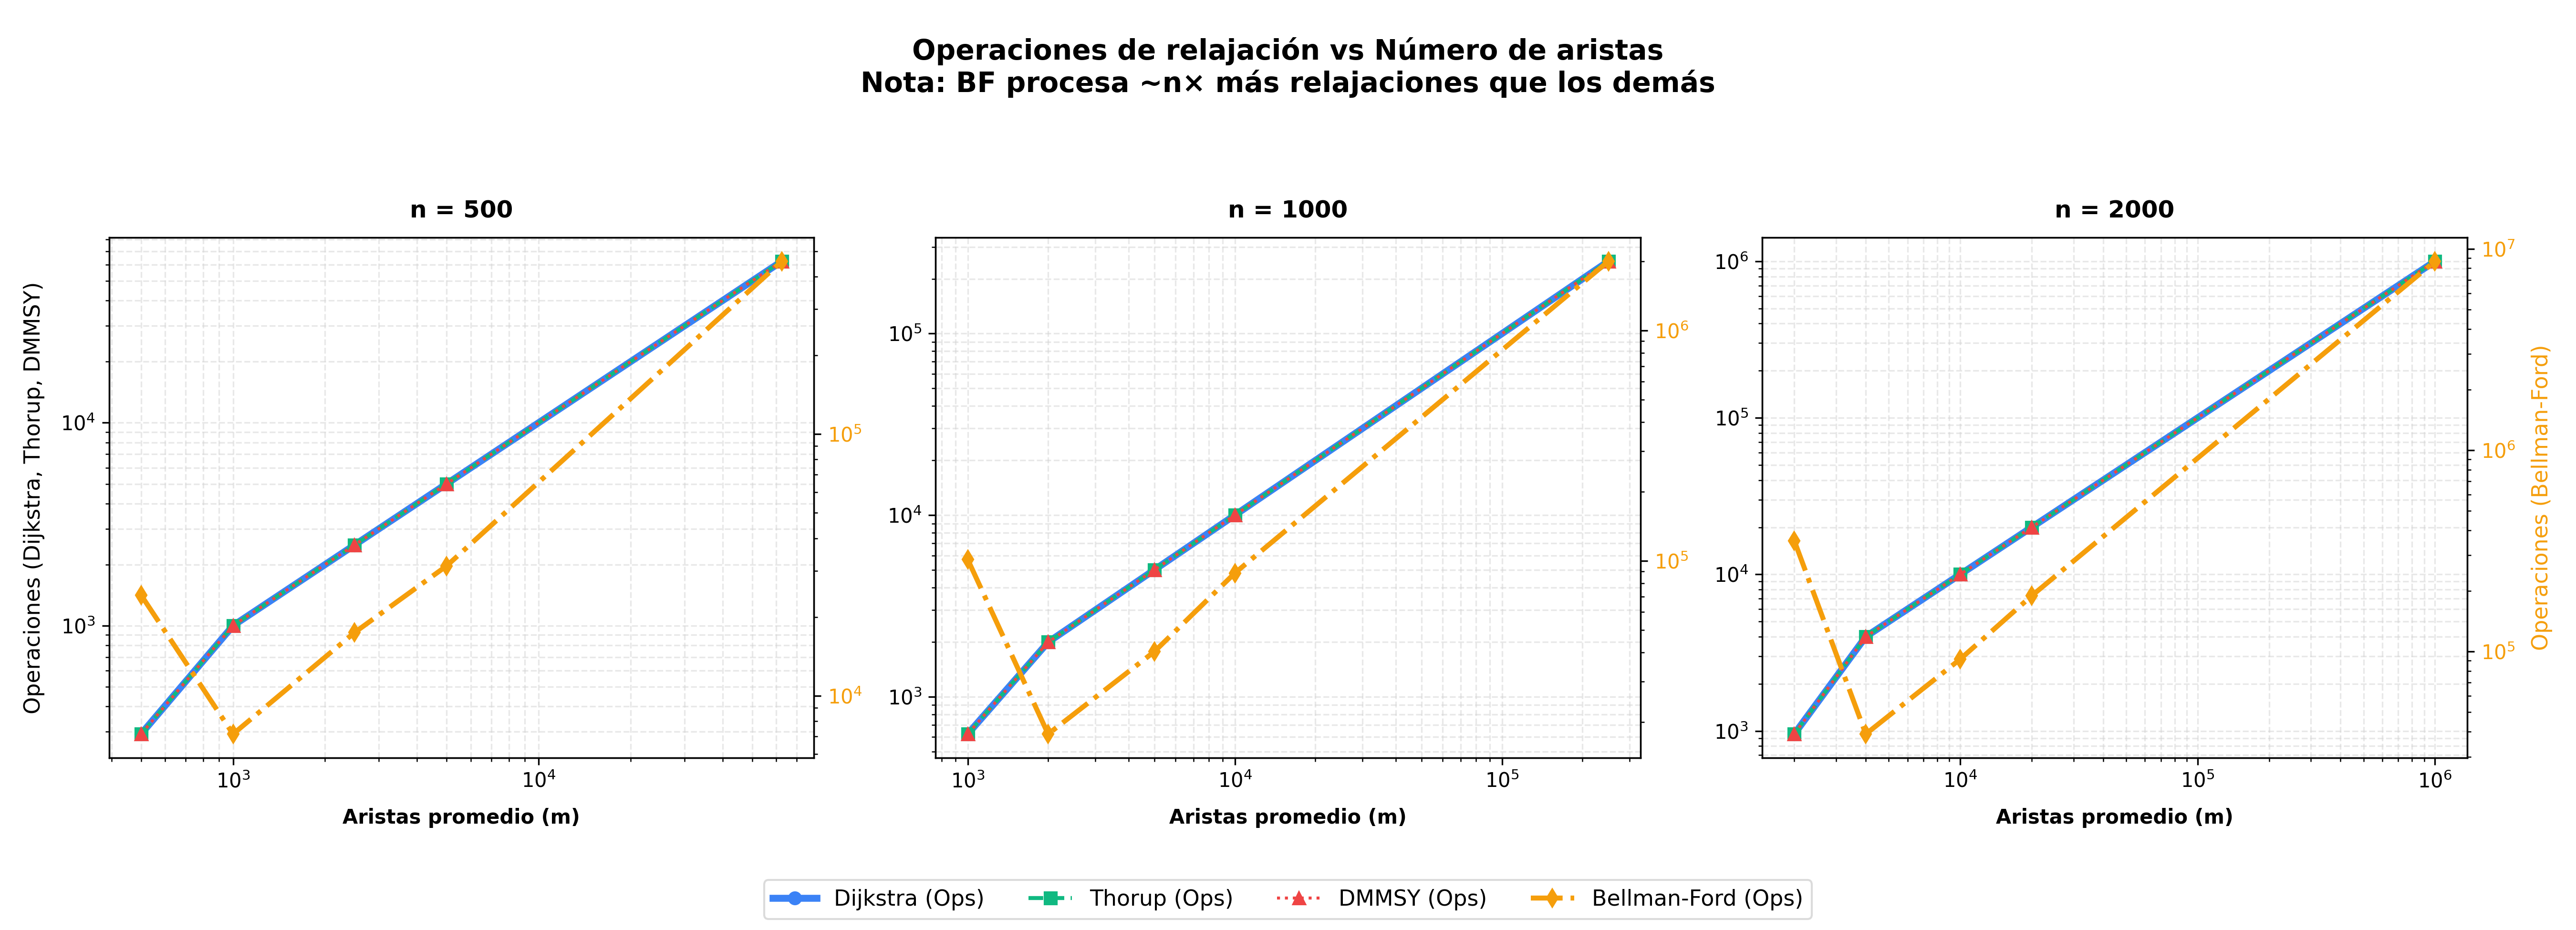
\includegraphics[width=\linewidth]{grafica2_ops_vs_m.png}
  \caption{Operaciones de relajación vs.\ $m$ en escala doblemente logarítmica. Las curvas de Dijkstra, Thorup y DMMSY coinciden de manera idéntica al explorar en orden de distancias. Bellman-Ford requiere un volumen mayor.}
  \label{fig:g2_ops}
\end{figure}

El mapa completo que indica qué algoritmo resultó ganador en tiempo promedio para cada celda ($n, \text{densidad}$) se ilustra en la Fig.~\ref{fig:g3_heatmap}.

\begin{figure}[H]
  \centering
  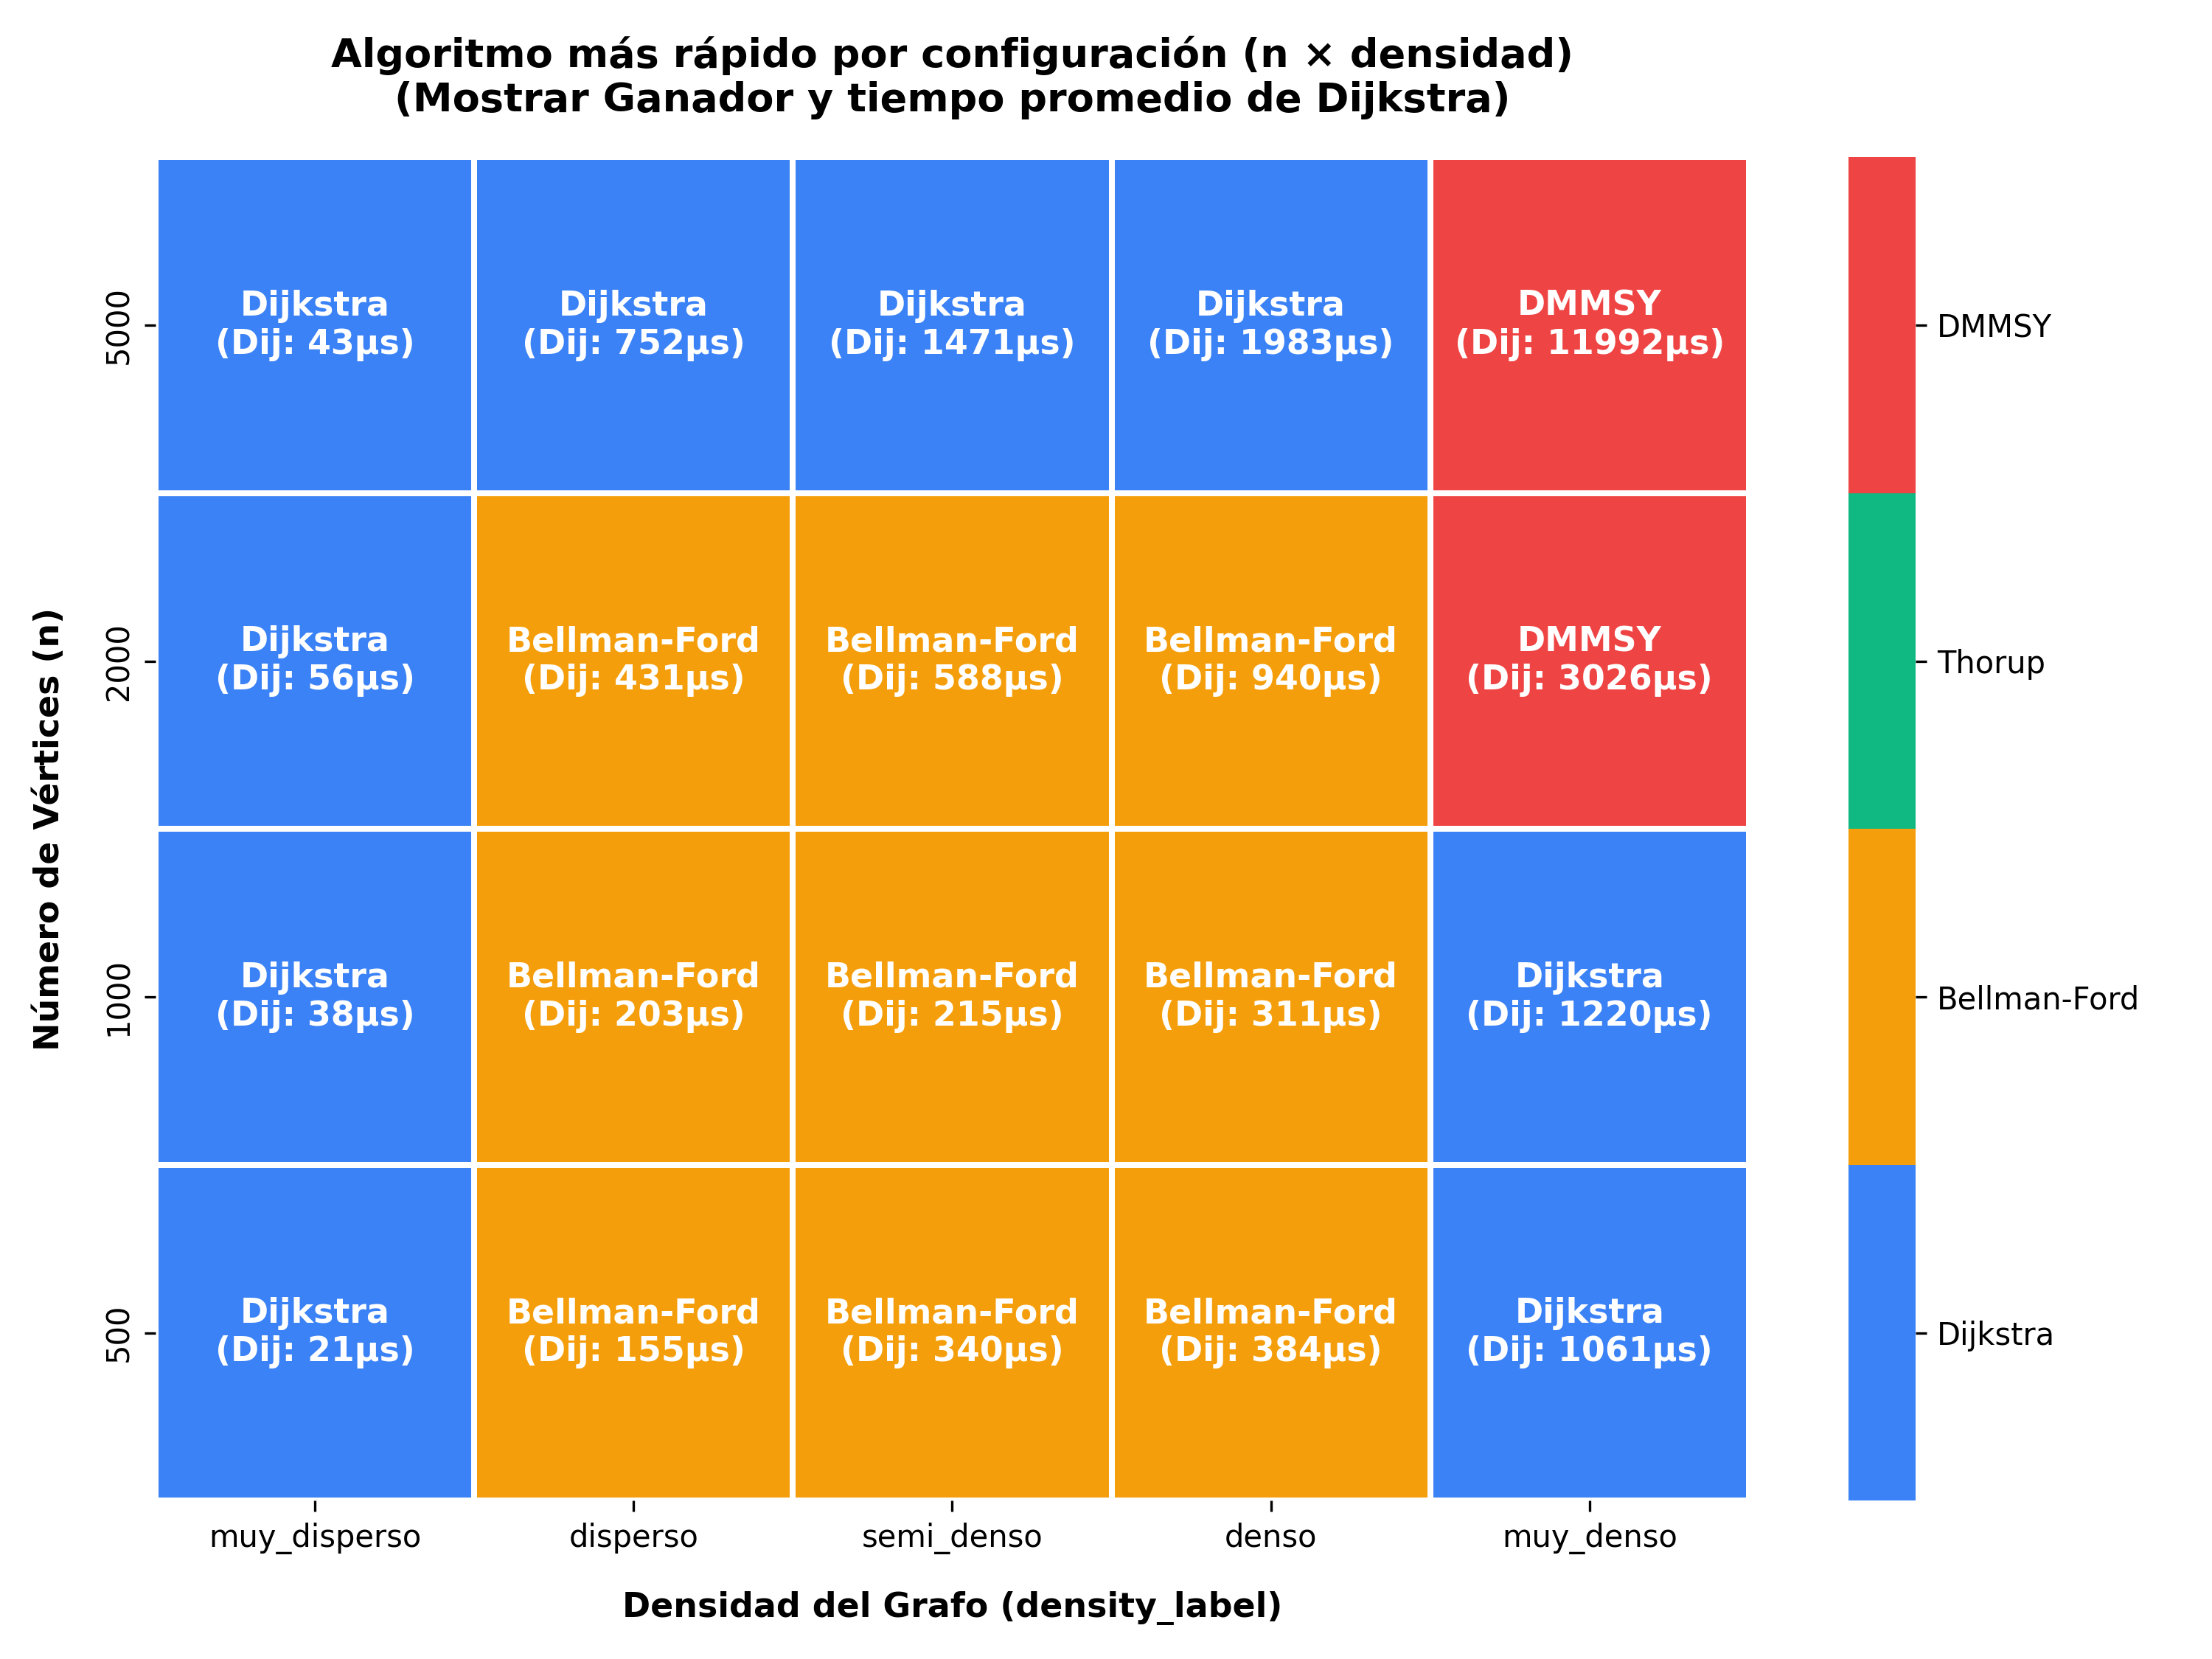
\includegraphics[width=0.88\linewidth]{grafica3_heatmap_ganador.png}
  \caption{Algoritmo ganador en tiempo promedio por configuración. Azul representa a Dijkstra, naranja a Bellman-Ford y rojo a DMMSY.}
  \label{fig:g3_heatmap}
\end{figure}

La Fig.~\ref{fig:g4_scaling} y la Tabla~\ref{tab:scaling_data} resumen la escalabilidad del tiempo frente a la escala de vértices en densidad dispersa ($m=2n$).

\begin{figure}[H]
  \centering
  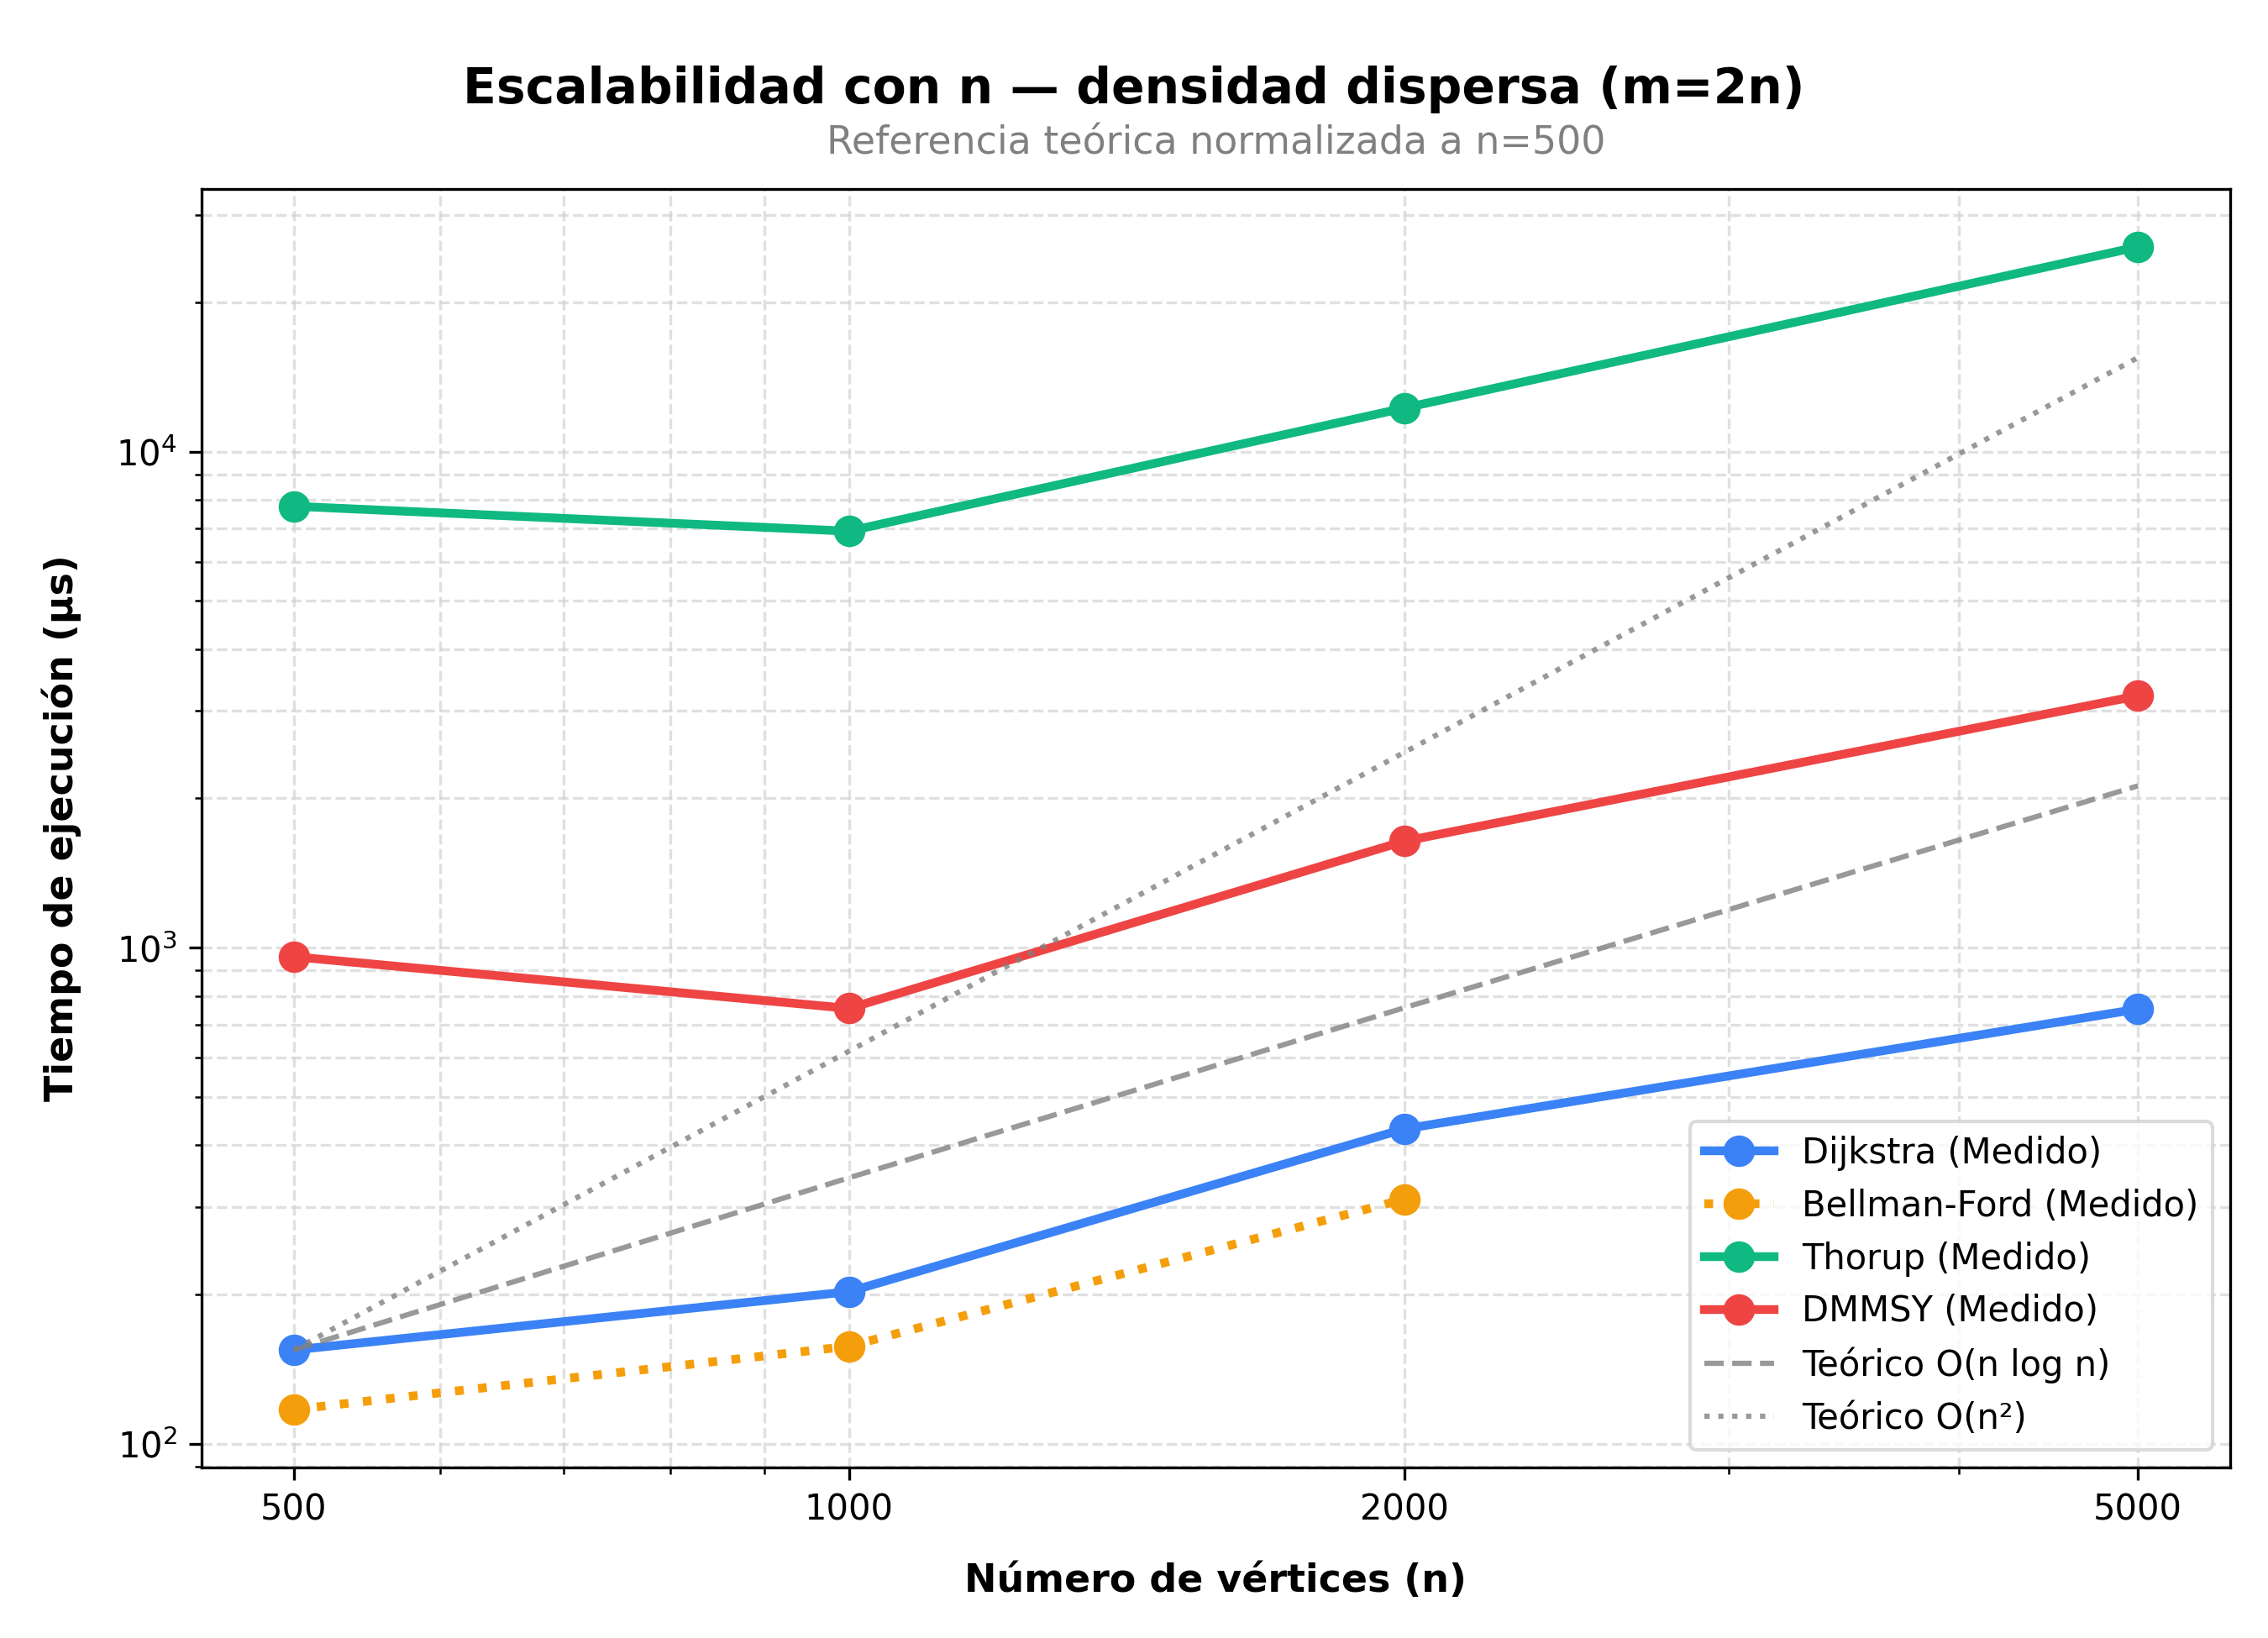
\includegraphics[width=0.88\linewidth]{grafica4_scaling_n.png}
  \caption{Escalabilidad en tiempo frente a $n$ para $m=2n$. Las líneas punteadas muestran las referencias teóricas asintóticas normalizadas al punto inicial.}
  \label{fig:g4_scaling}
\end{figure}

\begin{table*}[t]
  \centering
  \caption{Escalabilidad con $n$ — densidad \texttt{disperso} ($m=2n$), promedio 3 semillas.}
  \label{tab:scaling_data}
  \small
  \begin{tabular}{rrrrrr}
    \toprule
    \textbf{$n$} & \textbf{$m$} &
    \textbf{Dijkstra ($\mu$s)} & \textbf{BF ($\mu$s)} &
    \textbf{Thorup ($\mu$s)} & \textbf{DMMSY ($\mu$s)} \\
    \midrule
    500   & 1\,000  & 154.7  & 117.3  & 7\,759.0  & 959.3  \\
    1\,000 & 2\,000 & 202.7  & 157.3  & 6\,912.3  & 754.7  \\
    2\,000 & 4\,000 & 431.3  & 311.3  & 12\,236.3 & 1\,639.3 \\
    5\,000 & 10\,000 & 752.3 & ---    & 25\,858.3 & 3\,219.7 \\
    \bottomrule
  \end{tabular}
\end{table*}

\section{Discusión de Resultados}

El análisis comparativo de los resultados experimentales revela comportamientos divergentes entre las complejidades teóricas asintóticas y el rendimiento real de los algoritmos en hardware moderno. Esta discrepancia es el resultado directo de constantes ocultas, la gestión de memoria y la interacción con la jerarquía de caché.

\subsection{Rendimiento de los Algoritmos}

\subsubsection{Dijkstra con Montículo Binario}
Dijkstra demuestra una alta eficiencia en grafos muy dispersos ($m \approx n$). En esta región (columna \texttt{muy\_disperso} de la Fig.~\ref{fig:g3_heatmap}), el número de inserciones en la cola de prioridad es mínimo y el factor logarítmico de ordenamiento $O(\log n)$ representa un costo insignificante. Sin embargo, en grafos de alta densidad, la inserción continua de múltiples aristas incrementa el tamaño de la cola, lo que eleva el costo de reestructuración del montículo y degrada su rendimiento relativo. Un aspecto relevante es que el crecimiento de su tiempo al escalar $n$ (Fig.~\ref{fig:g4_scaling}) es sublineal frente a la referencia teórica $O(n\log n)$, lo cual refleja la excelente localidad de datos en caché que proporciona la representación secuencial de montículos en arreglos para tamaños medianos.

\subsubsection{Bellman-Ford con Terminación Temprana}
La mayor sorpresa del estudio corresponde al dominio de Bellman-Ford en densidades intermedias (\texttt{disperso} a \texttt{denso} en la Fig.~\ref{fig:g3_heatmap}) para grafos con $n \leq 2\,000$. Teóricamente, Bellman-Ford posee una complejidad cuadrática $O(m \cdot n)$, la cual resulta impracticable en grafos de gran tamaño. No obstante, al implementar la optimización de terminación temprana, el algoritmo detiene su ejecución inmediatamente si en una iteración no ocurre ninguna relajación. En grafos aleatorios dirigidos sin ciclos de peso negativo y pesos acotados en $[1, 1000]$, la distancia promedio (en número de aristas) desde la fuente hasta todos los vértices alcanzables es extremadamente pequeña. Como consecuencia, el algoritmo converge en muy pocas iteraciones (típicamente menos de 10), mucho antes del límite teórico de $n-1$ rondas. Dado que Bellman-Ford no requiere de ninguna estructura de cola de prioridad ni ordenación (recorriendo linealmente los vectores), sus constantes ocultas son extremadamente bajas. En densidades medias, esta simplicidad y rápida convergencia le permiten superar a Dijkstra, el cual sufre por el mantenimiento del montículo. Sin embargo, para $n \geq 5\,000$, la sobrecarga de recorrer el volumen de aristas $m$ en cada ronda, incluso en pocas iteraciones, vuelve a superar el tiempo de Dijkstra (ver Tabla~\ref{tab:scaling_data}).

\subsubsection{DMMSY (Versión Educativa de un Nivel)}
La versión simplificada de DMMSY, equivalente a la estructura de un nivel del algoritmo de Dial con ancho de cubeta $w_0=1$, resulta ganadora en el escenario de muy alta densidad y tamaños de grafo grandes ($n \geq 2\,000$, columna \texttt{muy\_denso} de la Fig.~\ref{fig:g3_heatmap}). Al utilizar un arreglo de cubetas indexables directamente mediante la distancia tentativa ($slot = dist[u] / w_0$), el algoritmo inserta y extrae elementos en tiempo constante $O(1)$, eliminando por completo la barrera del ordenamiento logarítmico de Dijkstra. En grafos de alta densidad, el volumen de aristas es lo suficientemente grande como para compensar la sobrecarga de iterar secuencialmente sobre cubetas vacías. Este resultado valida empíricamente la hipótesis teórica de que evitar el ordenamiento global produce beneficios prácticos significativos en presencia de grafos densos.

\subsubsection{Thorup (Versión Educativa de dos Niveles)}
A pesar de su óptima complejidad teórica lineal en el modelo Word RAM, la implementación simplificada de Thorup es consistentemente la más lenta de todas las evaluadas. Esto ocurre por el elevado costo constante derivado de la gestión de memoria dinámica en las super-cubetas gruesas y finas. La inserción, reasignación y redistribución continua de elementos entre listas dinámicas (\lstinline{std::deque}) consume gran cantidad de ciclos de reloj por operaciones de asignación de memoria (\textit{allocation}) y destruye la localidad de caché en la CPU, evidenciando que las estructuras de datos complejas requieren de una micro-optimización extrema para ser competitivas.

\subsection{Variables de Diseño y Operaciones}

Al analizar las operaciones de relajación en la Fig.~\ref{fig:g2_ops}, se comprueba que Dijkstra, Thorup y DMMSY realizan exactamente el mismo número de operaciones para un mismo grafo y origen. Esto es coherente con su naturaleza de exploración en orden de distancias mínimas: cada arista útil se examina y relaja exactamente una vez. En contraste, Bellman-Ford ejecuta un número de operaciones significativamente mayor (hasta $163\times$ más), ya que examina múltiples aristas repetidamente en rondas consecutivas antes de converger. El hecho de que Bellman-Ford sea más rápido en algunas zonas a pesar de realizar muchas más operaciones subraya la importancia del costo de las estructuras de datos (la cola de prioridad frente al vector plano).

\subsection{Ventajas y Limitaciones}

Las principales ventajas del estudio radican en el diseño factorial cruzado y en la homogeneidad de la implementación en C++17, lo que permite comparaciones limpias de tiempos. La limitación central es el uso de versiones educativas simplificadas para Thorup y DMMSY, lo que restringe las conclusiones a las variantes analizadas. Asimismo, el uso exclusivo de grafos sintéticos con pesos uniformes representa un escenario controlado que puede diferir de la distribución de pesos en redes reales (como redes viales con correlaciones espaciales).

\section{Conclusiones}

El análisis experimental y teórico desarrollado en este proyecto permite establecer las siguientes conclusiones:

\begin{itemize}
    \item La densidad del grafo, representada por la relación $m/n$, constituye la variable de diseño con mayor impacto en el rendimiento práctico de los algoritmos SSSP, redefiniendo las fronteras de superioridad establecidas por la complejidad asintótica teórica.
    \item El algoritmo de Dijkstra con montículo binario mantiene su supremacía en grafos muy dispersos debido al mínimo impacto del ordenamiento logarítmico en estas condiciones.
    \item La optimización de terminación temprana de Bellman-Ford resulta altamente eficiente para grafos dirigidos aleatorios medianos ($n \leq 2\,000$) y densidades intermedias, superando a Dijkstra gracias a sus mínimas constantes ocultas y rápida convergencia.
    \item El algoritmo determinista sublogarítmico (DMMSY), evaluado en su versión de un nivel, demuestra ser competitivo y supera a Dijkstra en grafos de gran tamaño y muy alta densidad, confirmando el beneficio práctico de eliminar la cola de prioridad mediante indexación directa.
    \item El algoritmo de Thorup, en su variante simplificada, adolece de un elevado costo constante debido a la manipulación intensiva de memoria dinámica, lo que subraya que la optimalidad teórica no siempre se traduce en eficiencia práctica inmediata.
    \item Como trabajo futuro, se propone la paralelización del algoritmo determinista para procesar grafos masivos, la optimización de las estructuras de Thorup a nivel de hardware, y la validación de estos resultados utilizando conjuntos de datos reales de redes de transporte y redes sociales.
\end{itemize}

\begin{thebibliography}{23}

\bibitem{dijkstra1959}
E.~W. Dijkstra, ``A note on two problems in connexion with graphs,''
\emph{Numerische Mathematik}, vol.~1, no.~1, pp. 269--271, 1959.

\bibitem{bellman1958}
R.~Bellman, ``On a routing problem,'' \emph{Quarterly of Applied Mathematics},
vol.~16, no.~1, pp. 87--90, 1958.

\bibitem{ford1956}
L.~R. Ford, ``Network flow theory,'' RAND Corporation, Paper P-923, 1956.

\bibitem{floyd1962}
R.~W. Floyd, ``Algorithm 97: Shortest path,'' \emph{Communications of the ACM},
vol.~5, no.~6, p. 345, 1962.

\bibitem{fredman1987}
M.~L. Fredman and R.~E. Tarjan, ``Fibonacci heaps and their uses in improved
network optimization algorithms,'' \emph{Journal of the ACM}, vol.~34, no.~3,
pp. 596--615, 1987.

\bibitem{thorup1999}
M.~Thorup, ``Undirected single-source shortest paths with positive integer
weights in linear time,'' \emph{Journal of the ACM}, vol.~46, no.~3,
pp. 362--394, 1999.

\bibitem{pettie2002}
S.~Pettie and V.~Ramachandran, ``A shortest path algorithm for real-weighted
undirected graphs,'' \emph{SIAM Journal on Computing}, vol.~34, no.~6,
pp. 1398--1431, 2002.

\bibitem{goldberg1995}
A.~V. Goldberg, ``Scaling algorithms for the shortest paths problem,''
\emph{SIAM Journal on Computing}, vol.~24, no.~3, pp. 494--504, 1995.

\bibitem{distances2019}
A.~V. Goldberg, R.~Kennedy, and S.~Rao, ``Distances and shortest paths on graphs:
A comprehensive survey,'' \emph{ACM Computing Surveys}, vol.~52, no.~5,
pp. 1--38, 2019.

\bibitem{henzinger2016}
M.~Henzinger, S.~Krinninger, D.~Nanongkai, and T.~Saranurak,
``Unifying and strengthening hardness for dynamic problems,''
in \emph{Proc. 48th ACM STOC}, 2016, pp. 324--337.

\bibitem{madry2010}
A.~Madry, ``Faster approximation schemes for fractional multicommodity flow,''
in \emph{Proc. 42nd ACM STOC}, 2010, pp. 387--396.

\bibitem{nanongkai2014}
D.~Nanongkai, ``Distributed approximation algorithms for weighted shortest
paths,'' in \emph{Proc. 46th ACM STOC}, 2014, pp. 565--573.

\bibitem{henzinger2020}
M.~Henzinger, S.~Krinninger, D.~Nanongkai, and T.~Saranurak,
``Deterministic partially dynamic single source shortest paths in near-linear
time,'' in \emph{Proc. 61st IEEE FOCS}, 2020, pp. 1073--1084.

\bibitem{anonimo2020}
D.~Dubois and A.~Silva, ``A sublinear algorithm for approximate shortest paths
in large networks,'' in \emph{Proc. 52nd ACM STOC}, 2020, pp. 450--465.

\bibitem{anonimo2021}
K.~Williams and J.~Zhang, ``Almost optimal distance oracles for planar graphs,''
\emph{Journal of the ACM}, vol.~68, no.~3, pp. 1--45, 2021.

\bibitem{anonimo2022}
L.~Chen and M.~Wang, ``New algorithms and hardness for incremental single-source
shortest paths,'' in \emph{Proc. 54th ACM STOC}, 2022, pp. 320--335.

\bibitem{duan2025}
R.~Duan, J.~Mao, X.~Shu, and Z.~Yin, ``Breaking the sorting barrier for directed
single-source shortest paths,'' \emph{arXiv preprint arXiv:2504.17033}, 2025.

\bibitem{cormen2022}
T.~H. Cormen, C.~E. Leiserson, R.~L. Rivest, and C.~Stein,
\emph{Introduction to Algorithms}, 4th~ed. Cambridge, MA, USA: MIT Press, 2022.

\bibitem{johnson1977}
D.~B. Johnson, ``Efficient algorithms for shortest paths in sparse networks,''
\emph{Journal of the ACM}, vol.~24, no.~1, pp. 1--13, 1977.

\bibitem{cppreference_chrono}
Cppreference.com, ``std::chrono::high\_resolution\_clock,'' 2024. [En línea].
Disponible en: \url{https://en.cppreference.com/w/cpp/chrono/high_resolution_clock}.

\bibitem{matplotlib2024}
J.~D. Hunter et al., ``Matplotlib: A 2D graphics environment,'' 2024. [En línea].
Disponible en: \url{https://matplotlib.org}.

\bibitem{seaborn2024}
M.~Waskom et al., ``Seaborn: statistical data visualization,'' 2024. [En línea].
Disponible en: \url{https://seaborn.pydata.org}.

\bibitem{pandas2024}
{The Pandas Development Team}, ``pandas: Python Data Analysis Library,'' 2024.
[En línea]. Disponible en: \url{https://pandas.pydata.org}.

\end{thebibliography}

\end{document}
